\documentclass[conference]{IEEEtran}
\IEEEoverridecommandlockouts

\usepackage{cite}
\usepackage{tabularx}
\usepackage{booktabs}
\usepackage{amsmath,amssymb,amsfonts}
\usepackage{algorithmic}
\usepackage{graphicx}
\usepackage{textcomp}
\usepackage{xcolor}

\def\BibTeX{{\rm B\kern-.05em{\sc i\kern-.025em b}\kern-.08em
    T\kern-.1667em\lower.7ex\hbox{E}\kern-.125emX}}

\begin{document}

\title{Formación de Equipos Multiples con Sociometría}

\author{
    \IEEEauthorblockN{Ignacio Martínez Hernández}
    \IEEEauthorblockA{\textit{Doctorado Sistemas en Ingeniería} \\
        \textit{Universidad de Talca}\\
        Talca, Chile \\
        imartinez17@alumnos.utalca.cl}
}

\maketitle

\begin{abstract}
    %La asignación de personal a múltiples proyectos es un desafío complejo en la gestión organizacional, que requiere un equilibrio entre las competencias técnicas y la cohesión social de los equipos. Este trabajo aborda el Problema de Formación de Múltiples Equipos (MTFP) mediante un modelo de Programación No Lineal Entera Mixta (MINLP). El modelo propuesto maximiza una métrica de eficiencia global que integra la afinidad sociométrica entre los individuos, los requerimientos de habilidades de cada proyecto y su prioridad estratégica. La implementación se realizó en Python utilizando Pyomo, con el solver Bonmin para la resolución. Los resultados experimentales sobre instancias sintéticas demuestran la validez y robustez del enfoque: el modelo encuentra soluciones óptimas validadas contra un método de fuerza bruta, escala eficientemente para problemas de tamaño realista y gestiona adecuadamente escenarios con altas tasas de afinidades negativas y requerimientos inviables. Se concluye que el modelo es una herramienta de apoyo a la decisión práctica y efectiva para formar equipos más cohesivos y productivos.
    La asignación de personal a múltiples proyectos es un desafío complejo en la gestión organizacional, que requiere un equilibrio entre las competencias técnicas y la cohesión social de los equipos. Este trabajo aborda el Problema de Formación de Múltiples Equipos (MTFP) mediante un modelo de Programación No Lineal Entera Mixta (MINLP). El modelo propuesto maximiza una métrica de eficiencia global que integra la afinidad sociométrica entre los individuos, los requerimientos de habilidades de cada proyecto y su prioridad estratégica. La implementación se realizó en Python utilizando Pyomo, con el solver Bonmin para la resolución. Los resultados experimentales sobre instancias sintéticas demuestran la validez y robustez del enfoque: el modelo encuentra soluciones óptimas validadas contra un método de fuerza bruta, escala eficientemente para problemas de tamaño realista y gestiona requerimientos inviables mediante un enfoque de relajación que identifica y cuantifica los déficits de habilidades, ofreciendo soluciones parciales accionables. Se concluye que el modelo es una herramienta de apoyo a la decisión práctica y efectiva para formar equipos más cohesivos y productivos.
\end{abstract}

\begin{IEEEkeywords}
    Formación de equipos, optimización, programación no lineal entera mixta, sociometría, Pyomo, Bonmin.
\end{IEEEkeywords}

\section{Introducción}
La formación de equipos multidisciplinarios es un desafío fundamental y recurrente en la gestión organizacional, especialmente al ejecutar múltiples proyectos simultáneamente en campos diversos como ingeniería, medicina o desarrollo de software. La eficiencia de estos equipos no solo radica en las habilidades técnicas individuales, sino crucialmente en la cohesión social y la dinámica interpersonal \cite{gutierrez2016multiple}. La asignación óptima de individuos a proyectos es inherentemente compleja, pues debe considerar competencias específicas, relaciones interpersonales, y restricciones como el cumplimiento de cuotas de habilidades o preferencias de colaboración.
Por lo tanto, es esencial abordar este problema de manera sistemática y formal, lo que nos lleva a modelar el Problema de Formación de Múltiples Equipos (MTFP) mediante un enfoque matemático. Este modelo no solo busca optimizar la asignación de recursos humanos a proyectos, sino también integrar las dimensiones técnicas y sociales para maximizar la eficiencia global del sistema organizacional.
Se aborda el Problema de Formación de Múltiples Equipos (MTFP) utilizando un modelo matemático para formalizar la toma de decisiones bajo restricciones.
El objetivo es asignar recursos humanos a múltiples proyectos, considerando tanto las habilidades técnicas requeridas como la cohesión social entre los miembros del equipo. Este enfoque busca maximizar la eficiencia organizacional al equilibrar las necesidades de los proyectos con las dinámicas interpersonales, proporcionando una herramienta útil para la gestión de equipos en entornos complejos y cambiantes.
El trabajo se estructura de la siguiente manera: en primer lugar, se presenta la metodología adoptada para abordar el problema, seguida de una descripción del entorno modelado y las consideraciones realizadas. Posteriormente, se define formalmente el modelo de optimización, incluyendo conjuntos, parámetros, variables de decisión, función objetivo y restricciones. Finalmente, se discuten las implicaciones de las simplificaciones realizadas y se presenta la implementación computacional del modelo utilizando Pyomo y el solver Bonmin, adecuado para problemas de optimización no lineal entera mixta.

\section{Metodología}

El enfoque propuesto para abordar el problema de formación de equipos multiples se divide en cuatro fases principales y conectadas entre sí:

\begin{enumerate}
    \item \textbf{Modelado del problema:} Se define formalmente el problema de asignación de recursos humanos a múltiples proyectos considerando la maximización de la afinidad social entre los miembros asignados. Este modelo incorpora variables y restricciones que aseguran asignaciones factibles y equilibradas, así como una función objetivo que mide la calidad social del equipo.

    \item \textbf{Generación de datos sintéticos:} Para evaluar y validar el modelo, se generan conjuntos de datos representativos de escenarios reales. Las relaciones sociales entre individuos y los requisitos de los proyectos se crean a partir de reglas controladas que simulan características típicas del contexto organizacional, asegurando diversidad en las instancias de prueba. Los datos se almacenan en formato JSON para facilitar su reutilización y análisis.

    \item \textbf{Implementación computacional:} Se emplea Pyomo\cite{pyomo_hart2011}, un lenguaje de modelado algebraico en Python, para construir el modelo de optimización. La solución se obtiene mediante el solver Bonmin\cite{bonmin_bonami2008}, capaz de manejar problemas de optimización no lineal entera mixta, lo cual es necesario debido a la inclusión de asignaciones de tiempo fraccionarias y discretas. El sistema permite configurar el modelo mediante archivos externos, lo que facilita la adaptación a diferentes tamaños y características del problema sin necesidad de modificar la estructura del código.

          %\item \textbf{Resolución y análisis:} Se realizan experimentos numéricos sobre diversas instancias para evaluar la efectividad y escalabilidad del enfoque. Los resultados se analizan desde el punto de vista de la maximización de la afinidad social, la factibilidad de las soluciones y el comportamiento computacional, permitiendo identificar fortalezas y áreas de mejora del modelo.
    \item \textbf{Resolución y análisis:} Se realizan experimentos numéricos sobre diversas instancias para evaluar la efectividad y escalabilidad del enfoque. Los resultados se analizan desde el punto de vista de la maximización de la afinidad social y la factibilidad de las soluciones. Se incluye un procedimiento de relajación para gestionar casos inviables, permitiendo identificar fortalezas y áreas de mejora del modelo.
\end{enumerate}



\section{Entorno Modelado y Consideraciones}

La formación de equipos en organizaciones que gestionan múltiples proyectos simultáneamente es un proceso complejo. Este se ve influenciado por numerosos factores técnicos, humanos, económicos y temporales. En la práctica, cada persona puede poseer múltiples habilidades, tener disponibilidad variable, y las interacciones sociales dentro de los equipos pueden evolucionar con el tiempo y el contexto del proyecto. A esto se suman las restricciones presupuestarias, los plazos de entrega y las dependencias técnicas entre proyectos, lo que agrega capas adicionales de complejidad que dificultan una modelación completa y exacta del sistema.

Para abordar el problema de manera manejable, el modelo propuesto incorpora ciertas simplificaciones. Se asume que cada persona tiene una única habilidad principal y puede ser asignada parcialmente a uno o más proyectos, representando así una disponibilidad fraccionada normalizada a su jornada laboral completa. Cada proyecto, a su vez, requiere al menos cierta cantidad de personas con cada tipo de habilidad específica, estableciendo así los requerimientos básicos para su desarrollo. Se considera además la existencia de una \textit{matriz de afinidad social} \cite{gutierrez2016multiple}, que refleja las relaciones positivas, negativas o neutras entre los miembros del equipo, la cual permanece fija durante el proceso de asignación. Por último, se asume que los proyectos son independientes entre sí, sin compartir recursos ni tener dependencias técnicas o temporales.

Para capturar de manera simplificada la importancia relativa o prioridad de cada proyecto dentro del conjunto, se asocia a cada uno un valor numérico denominado \textit{peso}. Este \textit{peso} sintetiza aspectos como la relevancia estratégica, el impacto económico, la urgencia derivada de retrasos o la criticidad en los procesos organizacionales. De esta forma, aunque el modelo no detalla todas las complejidades específicas de cada proyecto, el \textit{peso} permite ajustar la asignación y evaluación de equipos considerando la prioridad relativa, garantizando que proyectos más importantes tengan un mayor impacto en la solución final.

Es importante destacar que el modelo no contempla algunas características presentes en la realidad. Por ejemplo, no se considera que una persona pueda tener múltiples habilidades, ni se penaliza la asignación de recursos en exceso más allá de los requerimientos mínimos. Tampoco se incluyen restricciones económicas, plazos de entrega o dependencias técnicas entre proyectos. Asimismo, la matriz de afinidad social se mantiene estática y no evoluciona según experiencias previas o el contexto particular de cada proyecto.

Una consideración adicional para alinear el modelo con la práctica operativa es la restricción de las asignaciones de tiempo parcial a un conjunto discreto de fracciones permitidas (e.g., 0\%, 50\%, 100\%). Esto evita soluciones donde los individuos son asignados a múltiples proyectos con fracciones de tiempo muy pequeñas y poco realistas desde el punto de vista de la gestión y la dedicación efectiva (por ejemplo, una persona asignada al 10\% de su tiempo en diez proyectos diferentes). Esta discretización de las variables de asignación de tiempo transforma el problema en un modelo de Programación No Lineal Entera Mixta (MINLP).

Estas simplificaciones buscan un equilibrio entre la fidelidad del modelo y la factibilidad computacional y analítica. Aunque no capturan la totalidad de la complejidad real, permiten centrar el estudio en la interacción entre la adecuación técnica y la maximización de la afinidad social, aspectos centrales del problema de formación múltiple de equipos que se aborda en este trabajo. Estas consideraciones permiten acotar el espacio de soluciones y centrar el análisis en los aspectos de mayor relevancia para el problema.

\section{Definición del Modelo}

Para abordar formalmente el desafío de asignar personal a múltiples proyectos de manera que se consideren tanto las competencias técnicas como la dinámica social, se propone un modelo de optimización matemática. Debido a la necesidad de incorporar decisiones sobre fracciones de tiempo discretas, el modelo resultante es de Programación No Lineal Entera Mixta (MINLP). El objetivo central de este modelo es ayudar a los gestores a tomar decisiones de asignación que no solo cubran las necesidades de habilidades de cada proyecto, sino que también fomenten la cohesión y la sinergia dentro de los equipos formados, ponderando estas asignaciones según la importancia estratégica de cada proyecto. Este enfoque busca una solución que equilibre la eficiencia técnica con un ambiente de colaboración favorable, reconociendo que ambos son cruciales para el éxito organizacional.

En organizaciones que gestionan múltiples proyectos simultáneos, la asignación eficiente de personas a proyectos es crucial para el éxito. Cada individuo aporta una habilidad específica necesaria para cumplir tareas, mientras que las relaciones sociales entre personas influyen en la dinámica y desempeño del equipo. Además, los proyectos tienen distintas prioridades estratégicas que deben ser consideradas en la asignación.

Para capturar estas realidades, el modelo utiliza los siguientes elementos:

\begin{itemize}
    \item \textbf{Individuos} (\(\mathcal{H}\)): representan a los empleados o colaboradores disponibles, cada uno con una habilidad predominante.
    \item \textbf{Proyectos} (\(\mathcal{P}\)): iniciativas o tareas que requieren ciertos recursos humanos para completarse.
    \item \textbf{Habilidades} (\(\mathcal{K}\)): tipos de competencias técnicas o funcionales necesarias para cada proyecto.
    \item \textbf{Matriz de afinidad social} (\(s_{ij}\)): refleja la calidad de la relación entre personas, que puede ser positiva (cooperación), negativa (conflicto) o neutra.
    \item \textbf{Pesos de proyecto} (\(w_l\)): indican la importancia relativa o prioridad de cada proyecto dentro de la organización.
\end{itemize}

La variable de decisión \(x_{il}\) indica si la persona \(i\) es asignada al proyecto \(l\). La función objetivo busca maximizar un índice de eficiencia que pondera la prioridad de los proyectos con la cohesión social del equipo asignado, promoviendo tanto la satisfacción de los requerimientos técnicos como un ambiente colaborativo favorable.

Como se detalló en la sección de consideraciones previas, este modelo se fundamenta en simplificaciones clave, tales como la asignación de una única habilidad principal por individuo, la independencia entre proyectos y el carácter estático de la matriz de afinidad social durante el proceso de optimización.

\begin{figure}[htbp]
    \centering
    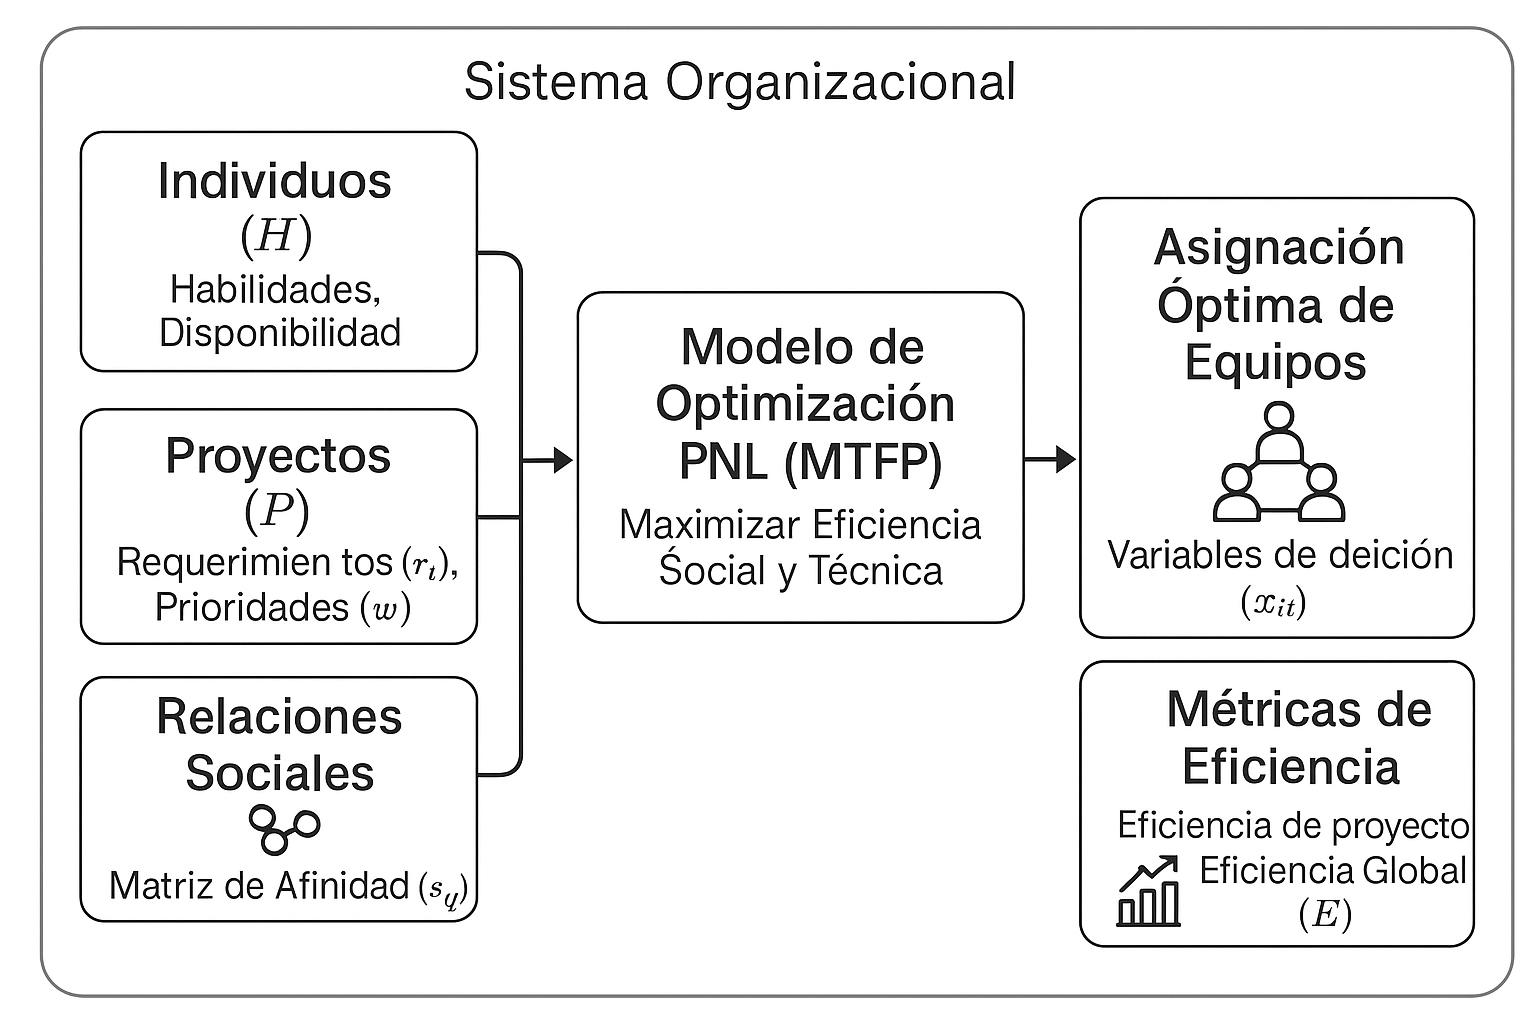
\includegraphics[width=0.8\linewidth]{diagrama_conceptual_mtfp.png}
    \caption{Modelo conceptual del Problema de Formación de Múltiples Equipos (MTFP), ilustrando sus componentes principales y flujos de información.}
    \label{fig:conceptual_model}
\end{figure}

\subsection{Conjuntos}
\begin{itemize}
    \item $\mathcal{H} = \{1, ..., n\}$: Individuos.
    \item $\mathcal{P} = \{1, ..., m\}$: Proyectos.
    \item $\mathcal{K} = \{1, ..., f\}$: Habilidades.
    \item $Q_a \subseteq \mathcal{H}$: Individuos con habilidad $a$.
    \item $\mathcal{D}$: conjunto de fracciones de tiempo discretas permitidas para la asignación (e.g., $\{0.0, 0.5, 1.0\}$).
\end{itemize}

\subsection{Parámetros}
\[
    s_{ij} =
    \begin{cases}
        1,  & \text{si la afinidad social entre } i \text{ y } j \text{ es positiva}, \\
        0,  & \text{si no existe relación o es neutral},                              \\
        -1, & \text{si la afinidad social es negativa}.
    \end{cases}
\]
\begin{itemize}
    \item $r_{al} \in \mathbb{R}$: cantidad mínima de dedicación (en personas) con habilidad $a$ requerida en el proyecto $l$.
    \item $w_l \in [0,1]$: peso o prioridad del proyecto $l$, con $\sum_{l \in \mathcal{P}} w_l = 1$.
\end{itemize}

\subsection{Variables de decisión}

%\begin{equation}
%    x_{il} \in [0,1]
%\end{equation}
%donde $x_{il}$ representa la fracción del tiempo o nivel de asignación del individuo $i$ al proyecto $l$.

Se introducen las siguientes variables de decisión:
\begin{itemize}
    \item \(y_{ild} \in \{0,1\}\): variable binaria que toma el valor 1 si al individuo \(i\) se le asigna la fracción de tiempo \(d \in \mathcal{D}\) para el proyecto \(l\), y 0 en caso contrario.
    \item \(x_{il}\): representa la fracción del tiempo total del individuo \(i\) asignada al proyecto \(l\). El valor de \(x_{il}\) se determina a partir de las variables \(y_{ild}\) y debe pertenecer al conjunto \(\mathcal{D}\).
\end{itemize}

\subsection{Función objetivo}

El modelo busca maximizar una métrica de eficiencia global que considera la calidad de las interacciones sociales dentro de cada equipo de proyecto, ponderada por la importancia relativa de cada proyecto. Para ello, primero definimos la eficiencia de cada proyecto \(l\), denotada como \(e_l\). Esta eficiencia intenta capturar cuán bien cohesionado socialmente está el equipo asignado al proyecto \(l\), en relación con su tamaño y requerimientos.

\begin{equation}
    e_l = \frac{1}{2} \left( 1 + \frac{\sum_{i,j \in \mathcal{H}} s_{ij} x_{il} x_{jl}}{\left(\sum_{a \in \mathcal{K}} r_{al}\right)^2} \right)
    \label{eq:efficiency_project_updated} % Changed label to avoid conflict if old one existed
\end{equation}


La interpretación de los componentes de \(e_l\) en relación con el fenómeno real es la siguiente:
\begin{itemize}
    \item \textbf{Afinidad social ponderada (\(\sum_{i,j \in \mathcal{H}} s_{ij} x_{il} x_{jl}\))}: Este término cuadrático es el núcleo de la medición de la cohesión social. El producto \(x_{il} x_{jl}\) representa el grado de interacción o colaboración conjunta entre las personas \(i\) y \(j\) en el proyecto \(l\). Si ambas personas están asignadas significativamente a dicho proyecto (valores altos de \(x_{il}\) y \(x_{jl}\)), su afinidad mutua \(s_{ij}\) (positiva, negativa o neutra) tiene un impacto magnificado en la cohesión del equipo. Esto refleja la realidad de que las relaciones interpersonales se vuelven más influyentes (para bien o para mal) cuando los individuos deben colaborar intensamente. La suma considera todas las posibles parejas de individuos.
    \item \textbf{Normalización (\(\left(\sum_{a \in \mathcal{K}} r_{al}\right)^2\))}: El denominador normaliza la afinidad social total del equipo. \(\sum_{a \in \mathcal{K}} r_{al}\) representa el "tamaño" o la "demanda total de personal" del proyecto \(l\). Al dividir por el cuadrado de esta suma, se obtiene una medida de cohesión relativa que es comparable entre proyectos de distintos tamaños. Sin esta normalización, los proyectos más grandes, que naturalmente tendrían más interacciones y, por lo tanto, una suma de afinidades potencialmente mayor en magnitud, podrían dominar la función objetivo independientemente de su cohesión \emph{relativa}. El uso del cuadrado puede interpretarse como una forma de escalar la afinidad con el número potencial de interacciones diádicas o la \emph{densidad} de requerimientos del proyecto. Esto ayuda a identificar equipos que son cohesivos en proporción a su escala, en lugar de favorecer simplemente a los equipos grandes.
    \item \textbf{Escalamiento (\( \frac{1}{2}(1 + \cdot) \))}: Esta transformación lineal asegura que la eficiencia \(e_l\) esté acotada en el intervalo \([0,1]\). Un valor de \(e_l = 1\) indicaría una cohesión social positiva perfecta en relación con el tamaño del proyecto, \(e_l = 0.5\) indicaría una cohesión neutra (afinidades positivas y negativas se cancelan o no hay afinidades significativas), y \(e_l = 0\) indicaría un conflicto social máximo. Este escalamiento facilita la interpretación de \(e_l\) como un índice normalizado de la calidad del ambiente social del equipo.
\end{itemize}

La fracción \(\sum_{i,j \in \mathcal{H}} s_{ij} x_{il} x_{jl}\) representa la afinidad social ponderada por el nivel de participación conjunta en el proyecto \(l\). Esta suma se normaliza dividiendo por el cuadrado del total de requerimientos del proyecto, es decir, \(\left(\sum_{a \in \mathcal{K}} r_{al}\right)^2\), lo que permite obtener una medida relativa de eficiencia que sea comparable entre proyectos de distintos tamaños. La expresión \( \frac{1}{2}(1 + \cdot) \) garantiza que la eficiencia esté acotada entre 0 y 1, incluso en presencia de afinidades negativas.

El problema de optimización consiste en maximizar la suma ponderada de las eficiencias de todos los proyectos. Esta función objetivo global, \(E\), se define como:

\begin{equation}
    \max E = \sum_{l \in \mathcal{P}} w_l \cdot e_l
    \label{eq:objective_total_updated} % Changed label
\end{equation}

Al maximizar \(E\), el modelo busca una asignación de personal que no solo forme equipos internamente cohesivos (maximizando cada \(e_l\)), sino que también priorice la calidad de estos equipos en los proyectos que son estratégicamente más importantes para la organización (debido al peso \(w_l\)). Por lo tanto, la solución óptima de este problema de PNL representa la mejor configuración de equipos posible, dadas las restricciones y los parámetros definidos, para alcanzar un equilibrio entre la cobertura de habilidades, la cohesión social y las prioridades organizacionales. Las decisiones del mundo real que este modelo ayuda a tomar son, fundamentalmente, a qué proyectos y en qué medida debe asignarse cada persona para lograr la máxima efectividad social y técnica del conjunto de equipos.

El uso del peso \(w_l\) en la función objetivo permite priorizar proyectos de acuerdo con su importancia relativa dentro del sistema, haciendo que aquellos más relevantes tengan una mayor influencia en la eficiencia total maximizada.

\subsection{Restricciones}
El modelo está sujeto a un conjunto de restricciones que reflejan las limitaciones y requerimientos operativos del mundo real en la asignación de personal:

\begin{align}
    \sum_{l \in \mathcal{P}} x_{il}  & \leq 1,                                     &  & \forall i \in \mathcal{H} \label{eq:constraint_capacity_updated}                              \\
    \sum_{i \in Q_a} x_{il}          & = r_{al},                                   &  & \forall a \in \mathcal{K}, \forall l \in \mathcal{P} \label{eq:constraint_skills_updated}     \\
    \sum_{d \in \mathcal{D}} y_{ild} & = 1,                                        &  & \forall i \in \mathcal{H}, \forall l \in \mathcal{P} \label{eq:constraint_force_one_fraction} \\
    x_{il}                           & = \sum_{d \in \mathcal{D}} d \cdot y_{ild}, &  & \forall i \in \mathcal{H}, \forall l \in \mathcal{P} \label{eq:constraint_define_x_from_y}
\end{align}

Estas restricciones se interpretan de la siguiente manera en el contexto del problema:

\begin{itemize}
    \item \textbf{Restricción de Capacidad Individual (Ecuación \ref{eq:constraint_capacity_updated})}: Esta restricción asegura que la asignación total de tiempo de un individuo \(i\) a todos los proyectos (\(\sum_{l \in \mathcal{P}} x_{il}\)) no exceda su disponibilidad total, que se normaliza a 1 (representando el 100\% de su tiempo laboral disponible). En el mundo real, esto significa que una persona no puede ser asignada a más trabajo del que puede realizar. Limita la sobrecarga de los individuos y refleja la finitud de los recursos humanos.

    \item \textbf{Restricción de Requerimientos de Habilidad por Proyecto (Ecuación \ref{eq:constraint_skills_updated})}: Esta restricción garantiza que para cada proyecto \(l\) y cada habilidad \(a\), la suma de las fracciones de tiempo de todas las personas (\(i \in Q_a\)) que poseen dicha habilidad y son asignadas al proyecto, sea \textbf{exactamente igual} a la cantidad requerida (\(r_{al}\)). Se optó por una igualdad estricta en lugar de una desigualdad (\(\geq\)) por una razón fundamental: evitar la sobreasignación de recursos. Si se permitiera una asignación mayor o igual, la función objetivo, en su afán por maximizar la afinidad social, tendería a asignar a todas las personas disponibles con afinidades positivas, incluso si exceden con creces los requerimientos técnicos. La igualdad impone un principio de eficiencia de recursos, asegurando que los equipos se dimensionen precisamente según las necesidades, lo que se alinea mejor con objetivos de control de costos y gestión práctica. Esta rigidez, sin embargo, es una de las principales causas de inviabilidad del modelo, lo que justifica la posterior introducción de un mecanismo de relajación.

    \item \textbf{Restricción de Selección Única de Fracción de Tiempo (Ecuación \ref{eq:constraint_force_one_fraction})}: Para cada par individuo-proyecto \((i,l)\), esta restricción asegura que se seleccione exactamente una fracción de tiempo \(d\) del conjunto de fracciones permitidas \(\mathcal{D}\). Esto implica que si un individuo no es asignado a un proyecto, la fracción seleccionada debe ser 0 (asumiendo que \(0 \in \mathcal{D}\)).

    \item \textbf{Restricción de Definición de Asignación (Ecuación \ref{eq:constraint_define_x_from_y})}: Esta restricción establece el valor de la variable de asignación \(x_{il}\) como la fracción de tiempo \(d \in \mathcal{D}\) que fue seleccionada mediante la variable binaria \(y_{ild}\). Garantiza que \(x_{il}\) solo tome valores del conjunto de fracciones discretas permitidas.
\end{itemize}

Estas restricciones son fundamentales para garantizar que la solución del modelo sea factible y refleje las realidades operativas de la organización. La primera asegura que no se asignen más recursos humanos de los disponibles, mientras que la segunda garantiza que cada proyecto cuente con el personal necesario para cumplir sus objetivos técnicos.



\section{Análisis del Modelo y Justificación de Simplificaciones}

El modelo de Formación de Múltiples Equipos (MTFP) presentado en este trabajo constituye una abstracción matemática del complejo proceso real de asignación de personal en entornos organizacionales. Para desarrollar una herramienta de optimización que sea computacionalmente tratable y útil en la práctica, se han incorporado ciertas simplificaciones. Estas decisiones de diseño distinguen al modelo del entorno real, que es inherentemente dinámico y está sujeto a una evolución constante.

\subsection{Representación Estática de un Proceso Dinámico}
La formación y gestión de equipos en el mundo real es un proceso continuo y dinámico. Las relaciones interpersonales evolucionan, las prioridades de los proyectos pueden cambiar y la disponibilidad de los individuos fluctúa. En contraste, el modelo matemático propuesto es inherentemente \textit{estático}. Proporciona una asignación óptima para un conjunto específico de parámetros (afinidades sociales, requerimientos de habilidades y pesos de proyectos) en un momento determinado.

Esta naturaleza estática se adopta para definir un problema de optimización bien delimitado que pueda resolverse de manera eficiente. La utilidad del modelo radica en su capacidad para ofrecer un punto de partida robusto para la asignación de equipos o para realizar reevaluaciones periódicas, en lugar de intentar una adaptación continua en tiempo real, lo cual requeriría un enfoque de modelado considerablemente más complejo.

\subsection{Parámetros Fijos y Dinámica Social}
El modelo opera con una matriz de afinidad social ($s_{ij}$) y unos pesos de proyecto ($w_l$) que se consideran fijos durante la ejecución del proceso de optimización. En la realidad organizacional, las afinidades sociales no son inmutables; pueden fortalecerse o debilitarse en función de las experiencias compartidas, los resultados de los proyectos o factores externos. De manera similar, las prioridades estratégicas de los proyectos pueden ser objeto de reevaluación.

La decisión de utilizar parámetros fijos es una simplificación necesaria para mantener la tratabilidad del modelo. Modelar la evolución completa de la dinámica social y las prioridades de los proyectos introduciría un nivel de complejidad que podría requerir enfoques basados en simulación o programación dinámica, alejándose del objetivo de proporcionar una herramienta de asignación inicial eficiente. Se espera que, en la práctica, el modelo se ejecute nuevamente con parámetros actualizados a medida que se disponga de nueva información sobre el estado del sistema (por ejemplo, tras evaluaciones de desempeño o cambios estratégicos).

\subsection{Ausencia de Mecanismos Internos de Retroalimentación y Control}
La gestión de equipos en un entorno real implica ciclos continuos de retroalimentación, monitoreo y ajuste. Si un equipo muestra un rendimiento inferior al esperado o surgen conflictos internos, los responsables de la gestión intervienen para realizar correcciones.

El modelo de optimización propuesto no incorpora tales bucles de retroalimentación ni mecanismos de control internos \textit{dentro de una única ejecución}. Resuelve el problema de asignación basándose en los datos de entrada proporcionados y no se autoajusta en función de un hipotético desempeño futuro o de la evolución de las interacciones.

Esta característica se debe a que el modelo está concebido como una \textit{herramienta de optimización} para un estado específico del sistema, no como una simulación completa del ciclo de vida de la gestión de equipos. Los procesos de control y retroalimentación del mundo real ocurrirían \textit{fuera} del ámbito de una ejecución individual del modelo. Estos procesos externos podrían, no obstante, informar la actualización de los parámetros de entrada para ejecuciones subsecuentes del modelo (por ejemplo, ajustando $s_{ij}$ basándose en la cohesión observada en los equipos o modificando $w_l$ según nuevos lineamientos estratégicos).

\subsection{Implicaciones para la Aplicación Práctica}
Las simplificaciones discutidas implican que el modelo es una herramienta potente para el \textit{apoyo a la toma de decisiones} en momentos específicos, más que un sistema autónomo de gestión continua. Su fortaleza reside en su capacidad para abordar la complejidad combinatoria inherente a la asignación de múltiples individuos a múltiples proyectos, considerando simultáneamente habilidades técnicas y factores sociales, a partir de la mejor información disponible en el momento de la ejecución.

El resultado del modelo debe interpretarse como una recomendación fundamentada, que posteriormente puede ser sometida a la revisión y el juicio experto de los gestores, e integrada dentro de los procesos organizacionales más amplios y dinámicos. Este enfoque equilibra el rigor matemático con la aplicabilidad operativa, facilitando la toma de decisiones informada sin pretender replicar toda la complejidad del sistema social real.


\section{Implementación Computacional}

Para resolver el modelo de optimización propuesto se utilizó \textbf{Pyomo}\cite{pyomo_hart2011}, un lenguaje de modelado algebraico en Python que permite definir variables, restricciones y funciones objetivo de forma declarativa. La elección de Pyomo responde a su flexibilidad para trabajar con modelos de optimización no lineales y su compatibilidad con diversos solucionadores. Dado que el modelo incorpora variables enteras (para la selección de fracciones de tiempo discretas) y una función objetivo no lineal, se clasifica como un problema de Programación No Lineal Entera Mixta (MINLP), para lo cual se utilizó el solver Bonmin\cite{bonmin_bonami2008}. El código fuente completo de esta implementación, incluyendo la generación de datos y la resolución del modelo, está disponible públicamente\footnote{El código fuente puede consultarse en: https://github.com/DarkNacho/Multiple-Team-Formation}.

\subsection{Descripción del proceso}

El sistema fue diseñado de forma modular, permitiendo que tanto los parámetros del problema como las instancias específicas se definan a través de archivos externos en formato \texttt{JSON}. Esta estructura facilita la reutilización del código y la adaptación del modelo a distintos escenarios, sin necesidad de alterar su núcleo.

La ejecución del modelo sigue los siguientes pasos:
\begin{enumerate}
    \item Carga de datos desde archivos \texttt{JSON} en caso de contar con un dataset real.
    \item Generación opcional de datos aleatorios para pruebas cuando no se disponga de un dataset real.
    \item Construcción del modelo en Pyomo, especificando variables (incluyendo las binarias para la selección de fracciones de tiempo), función objetivo y restricciones.
    \item Solución del modelo utilizando el solver \textbf{Bonmin}.
    \item Almacenamiento y análisis de los resultados obtenidos.
\end{enumerate}

\subsection{Configuración del Solver}

El solver Bonmin se integró mediante la interfaz proporcionada por Pyomo. Para esta implementación, se usaron sus parámetros por defecto, sin modificaciones adicionales.

\section{Resultados y Discusión}

Al interpretar la métrica de eficiencia del proyecto $e_l$, definida en la Ecuación \ref{eq:efficiency_project_updated}, es importante considerar una sutileza relacionada con la matriz de afinidad social $s_{ij}$. Como se describió anteriormente, un valor de $e_l=0.5$ se interpreta como un punto de cohesión neutra, donde las afinidades positivas y negativas se cancelan. Sin embargo, es una convención común o una implicación de la definición de $s_{ij}$ que la afinidad de un individuo consigo mismo, $s_{ii}$, sea 1. Si este es el caso, la diagonal de la matriz de afinidad contribuye positivamente a la suma $\sum_{i,j \in \mathcal{H}} s_{ij} x_{il} x_{jl}$.

Específicamente, el término $\sum_{i,j \in \mathcal{H}} s_{ij} x_{il} x_{jl}$ en el numerador de $e_l$ incluye la suma de los cuadrados de las asignaciones ponderadas por la auto-afinidad, es decir, $\sum_{i \in \mathcal{H}} s_{ii} x_{il}^2$. Si $s_{ii}=1$ para todo $i$, este componente es $\sum_{i \in \mathcal{H}} x_{il}^2$, que es inherentemente no negativo. Para que la eficiencia $e_l$ sea exactamente 0.5, la suma total $\sum_{i,j \in \mathcal{H}} s_{ij} x_{il} x_{jl}$ debe ser cero. Esto implica que la suma de las afinidades interpersonales (es decir, los términos donde $i \neq j$) no solo debe ser cero por sí misma, sino que debe ser suficientemente negativa para contrarrestar el término positivo $\sum_{i \in \mathcal{H}} x_{il}^2$.

En consecuencia, un equipo donde todas las relaciones \textit{interpersonales} son estrictamente neutras (es decir, $s_{ij}=0$ para todo $i \neq j$), y asumiendo $s_{ii}=1$, resultaría en un valor de $e_l$ ligeramente superior a 0.5, dado por:
\[ e_l = \frac{1}{2} \left( 1 + \frac{\sum_{i \in \mathcal{H}} x_{il}^2}{\left(\sum_{a \in \mathcal{K}} r_{al}\right)^2} \right) \]
Esta consideración no invalida la utilidad de $e_l$ como un indicador de la cohesión social del equipo, ni el rango de $[0,1]$. Simplemente refina la interpretación del punto $e_l=0.5$: este valor representa un estado donde las interacciones sociales negativas entre distintos miembros del equipo son lo suficientemente fuertes como para anular tanto las interacciones positivas entre otros miembros como la contribución basal positiva derivada de las auto-afinidades. La escala sigue siendo efectiva para comparar la cohesión relativa entre diferentes configuraciones de equipos. En lo que respecta al límite inferior de la escala, $e_l=0$, este se alcanzaría si el término de afinidad social total, $\sum_{i,j \in \mathcal{H}} s_{ij} x_{il} x_{jl}$, fuese igual a $-\left(\sum_{a \in \mathcal{K}} r_{al}\right)^2$. Considerando la contribución inherentemente positiva de las auto-afinidades (asumiendo $s_{ii}=1$), para que $e_l$ llegue a cero, la suma de las afinidades interpersonales negativas ($\sum_{i \neq j} s_{ij} x_{il} x_{jl}$) debe ser excepcionalmente fuerte, superando no solo las afinidades interpersonales positivas sino también la suma de $\sum_{i \in \mathcal{H}} x_{il}^2$. De hecho, para equipos muy pequeños (uno o dos miembros), incluso si todas las afinidades interpersonales fuesen -1 (y $s_{ii}=1$), el valor de $e_l$ no podría ser 0 (y, de hecho, se mantendría $\geq 0.5$) si existen requerimientos de proyecto ($\sum_{a \in \mathcal{K}} r_{al} > 0$), ya que la contribución positiva de las auto-afinidades no es superada en tal medida. Sin embargo, para equipos más grandes (tres o más miembros), es teóricamente posible que $e_l$ alcance el valor 0 si las interacciones negativas son suficientemente intensas y generalizadas. En la práctica, un valor de $e_l$ cercano a 0 siempre indicará un nivel de conflicto social extremadamente alto y perjudicial para el proyecto.

Este comportamiento teórico se confirma en los experimentos de robustez. Como se observa en la Tabla \ref{tab:robustez}, incluso en un escenario extremo donde el 100\% de las afinidades interpersonales son negativas, la eficiencia global resultante es de 22.22\%, un valor marcadamente superior a cero. Este resultado ilustra cómo la contribución basal positiva de las auto-afinidades ($s_{ii}=1$) impide que la eficiencia colapse a 0, incluso bajo un conflicto generalizado, ya que el modelo debe cumplir con los requerimientos técnicos del proyecto.

\par Para evaluar la efectividad, robustez y escalabilidad del modelo MINLP propuesto, se diseñó y ejecutó un plan de pruebas exhaustivo. Los experimentos se realizaron sobre un conjunto de instancias sintéticas, generadas para simular diversos escenarios organizacionales. A continuación, se presentan y discuten los resultados obtenidos en cada una de las baterías de pruebas.

\subsection{Validación de Correctitud}
Para verificar la correctitud del modelo MINLP, la primera fase de experimentación consistió en comparar sus resultados con los de un método de referencia que garantiza la optimalidad: un algoritmo de fuerza bruta. Este algoritmo explora sistemáticamente todas las asignaciones posibles para encontrar la solución óptima global. Se utilizaron instancias de tamaño reducido, donde la exploración exhaustiva es computacionalmente factible.

Los resultados, resumidos en la Tabla \ref{tab:correctitud}, muestran una coincidencia exacta entre la eficiencia global óptima encontrada por el solver Bonmin y la obtenida por el método de fuerza bruta en todos los casos de prueba, incluyendo escenarios con afinidades negativas.

\begin{table}[htbp]
    \centering
    \caption{Comparación de resultados entre el solver y fuerza bruta para validación.}
    \label{tab:correctitud}
    \begin{tabularx}{\linewidth}{@{}lccc@{}}
        \toprule
        \textbf{Instancia}               & \textbf{Eficiencia Global} & \textbf{Eficiencia Global} \\
        (Personas/Proyectos/Habilidades) & \textbf{Fuerza Bruta}      & \textbf{Solver}            \\
        \midrule
        2p / 1pr / 1sk (afin. pos)       & 100.00\%                   & 100.00\%                   \\
        3p / 2pr / 2sk (afin. mix)       & 100.00\%                   & 100.00\%                   \\
        4p / 2pr / 2sk (afin. nega)      & 75.00\%                    & 75.00\%                    \\
        6p / 1pr / 2sk (excedente)       & 75.00\%                    & 75.00\%                    \\
        \bottomrule
    \end{tabularx}
\end{table}

La perfecta correspondencia en los valores de la función objetivo, así como en las asignaciones de variables de decisión, confirma que el modelo está formulado correctamente y que el solver es capaz de encontrar la solución óptima global para problemas de baja dimensionalidad. Esta validación inicial es un paso crucial antes de proceder a evaluar la escalabilidad y el comportamiento del modelo en instancias de mayor tamaño.

\subsection{Análisis de Escalabilidad}
Se evaluó el comportamiento del modelo frente a instancias de tamaño creciente para medir su escalabilidad. Se generaron problemas con un número de personas desde 10 hasta 100, con un aumento proporcional en el número de proyectos y habilidades. Los resultados se resumen en la Tabla \ref{tab:escalabilidad}.

\begin{table}[htbp]
    \centering
    \caption{Resultados de las pruebas de escalabilidad.}
    \label{tab:escalabilidad}
    \begin{tabularx}{\linewidth}{@{}lccc@{}}
        \toprule
        \textbf{Instancia}               & \textbf{Eficiencia} & \textbf{Tiempo (s)} \\
        (Personas/Proyectos/Habilidades) & \textbf{Global}     &                     \\
        \midrule
        10p / 2pr / 2sk                  & 81.90\%             & 0.22                \\
        20p / 5pr / 4sk                  & 75.11\%             & 0.84                \\
        30p / 5pr / 4sk                  & 60.22\%             & 5.05                \\
        50p / 10pr / 8sk                 & 73.65\%             & 45.11               \\
        100p / 10pr / 8sk                & 67.86\%             & 622.19              \\
        \bottomrule
    \end{tabularx}
\end{table}

Como era de esperar, el tiempo de resolución aumenta de forma no lineal con el tamaño del problema, lo cual es característico de los problemas MINLP. Para la instancia más grande, con 100 personas, el modelo tardó poco más de 10 minutos en encontrar la solución óptima. Este resultado es prometedor, ya que demuestra que el modelo es capaz de resolver problemas de tamaño realista en un tiempo razonable.

\subsection{Impacto de la Discretización del Tiempo}
Se analizó cómo la granularidad de las fracciones de tiempo permitidas (\(\mathcal{D}\)) afecta la solución y el rendimiento. Se ejecutó la misma instancia (6 personas, 2 proyectos, 2 habilidades) con tres conjuntos de fracciones distintos. La Tabla \ref{tab:discretizacion} compara los resultados obtenidos por el solver Bonmin y el algoritmo de fuerza bruta.

\begin{table}[htbp]
    \centering
    \caption{Impacto de la discretización del tiempo en una instancia de 6p/2pr/2sk.}
    \label{tab:discretizacion}
    \begin{tabularx}{\linewidth}{@{}lccc@{}}
        \toprule
        \textbf{Fracciones Permitidas (\(\mathcal{D}\))} & \textbf{Eficiencia} & \textbf{Tiempo}     & \textbf{Tiempo}           \\
                                                         & \textbf{Global}     & \textbf{Solver (s)} & \textbf{Fuerza Bruta (s)} \\
        \midrule
        \{0, 1\}                                         & 88.89\%             & 0.18                & 0.04                      \\
        \{0, 0.5, 1\}                                    & 88.89\%             & 0.13                & 3.56                      \\
        \{0, 0.25, 0.5, 0.75, 1\}                        & 88.89\%             & 0.13                & 1407.97                   \\
        \bottomrule
    \end{tabularx}
\end{table}

Los resultados muestran que, para esta instancia particular, la eficiencia global óptima fue la misma en todos los escenarios, indicando que la solución óptima no requería asignaciones de tiempo parciales. Sin embargo, el análisis del tiempo de cómputo revela una diferencia crucial: mientras que el tiempo del solver se mantuvo estable y bajo, el tiempo del algoritmo de fuerza bruta creció de manera exponencial. Al aumentar la granularidad, el espacio de búsqueda para la fuerza bruta se expandió drásticamente, llevando el tiempo de ejecución de 0.04 segundos a más de 23 minutos.

Este experimento subraya dos puntos importantes: primero, la capacidad del modelo para manejar fracciones de tiempo finas es una característica clave para problemas más complejos donde las asignaciones parciales podrían ser necesarias para alcanzar la optimalidad. Segundo, demuestra la clara superioridad computacional del solver MINLP sobre un método de búsqueda exhaustiva, siendo indispensable para resolver problemas de tamaño realista de manera eficiente.

\subsection{Robustez ante Afinidades Negativas}
Para medir la capacidad del modelo de gestionar conflictos interpersonales, se crearon instancias con una proporción creciente de afinidades negativas, desde un 50\% hasta un 100\%. Los resultados (Tabla \ref{tab:robustez}) muestran que la eficiencia global disminuye drásticamente a medida que aumenta la proporción de afinidades negativas. Esto ocurre porque el modelo se ve forzado a asignar personas con conflictos para cumplir con los requerimientos técnicos de los proyectos.

\begin{table}[htbp]
    \centering
    \caption{Impacto de afinidades negativas en una instancia de 6p/2pr/2sk.}
    \label{tab:robustez}
    \begin{tabularx}{\linewidth}{@{}lcccc@{}}
        \toprule
        \textbf{Proporción Negativas} & \textbf{Eficiencia Global} \\
        \midrule
        50\%                          & 55.56\%                    \\
        60\%                          & 38.89\%                    \\
        80\%                          & 33.33\%                    \\
        90\%                          & 22.22\%                    \\
        100\%                         & 22.22\%                    \\
        \bottomrule
    \end{tabularx}
\end{table}

Este comportamiento demuestra que el modelo es sensible a la estructura social y penaliza fuertemente las configuraciones de equipos con alta conflictividad, tal como se esperaba. Para validar la calidad de la solución, el caso con 50\% de afinidades negativas se verificó mediante fuerza bruta, confirmando que la eficiencia del 55.56\% es óptima. Sin embargo, la fuerza bruta requirió 1441.19 segundos (aprox. 24 minutos) para encontrarla, en contraste con los 0.28 segundos del solver. Este resultado subraya la capacidad del modelo para encontrar soluciones óptimas de manera eficiente incluso en escenarios de alta conflictividad.

\subsection{Sensibilidad a la Prioridad de Proyectos}
Se evaluó si el modelo responde correctamente a los pesos (\(w_l\)) asignados a los proyectos. Se configuró una instancia con dos proyectos, variando sus pesos relativos. Los resultados se muestran en la Tabla \ref{tab:sensibilidad}.

\begin{table}[htbp]
    \centering
    \caption{Sensibilidad a la prioridad de proyectos en una instancia de 6p/2pr/2sk.}
    \label{tab:sensibilidad}
    \begin{tabularx}{\linewidth}{@{}lcccc@{}}
        \toprule
        \textbf{Pesos (P1, P2)} & \textbf{Eficiencia P1} & \textbf{Eficiencia P2} & \textbf{Eficiencia Global} \\
        \midrule
        (80\%, 20\%)            & 88.89\%                & 77.78\%                & 86.67\%                    \\
        (95\%, 5\%)             & 88.89\%                & 77.78\%                & 88.33\%                    \\
        \bottomrule
    \end{tabularx}
\end{table}

En ambos experimentos, el modelo asignó el mismo conjunto de personas a cada proyecto. Aunque la asignación no cambió, el resultado demuestra que el modelo prioriza correctamente, ya que la eficiencia global ponderada aumenta conforme se asigna mayor peso al proyecto con el equipo más cohesivo (Proyecto 1).

\subsection{Gestión de Casos Inviables y Relajación del Modelo}
Finalmente, se probó la robustez del modelo ante escenarios sin solución factible. Para ello, se implementó un enfoque de dos etapas. Primero, se intenta resolver el modelo estricto. Si el solver reporta que la instancia es inviable (\textit{infeasible}), se activa un segundo modelo relajado.

Este modelo relajado introduce variables de holgura (déficit) en la restricción de requerimientos de habilidad, permitiendo que no se cumplan por completo. Para asegurar que el modelo aún intente satisfacer la mayor cantidad de requerimientos posible, se modifica la función objetivo para incluir una fuerte penalización proporcional a la suma de todos los déficits.

Matemáticamente, se introduce una nueva variable de déficit \(\delta_{al} \geq 0\). La restricción de requerimientos (Ecuación \ref{eq:constraint_skills_updated}) se reemplaza por:
\begin{equation}
    \sum_{i \in Q_a} x_{il} + \delta_{al} = r_{al}, \quad \forall a \in \mathcal{K}, \forall l \in \mathcal{P}
    \label{eq:constraint_skills_relaxed}
\end{equation}

Y la función objetivo (Ecuación \ref{eq:objective_total_updated}) se modifica para penalizar este déficit:
\begin{equation}
    \max E_{\text{relajado}} = \left( \sum_{l \in \mathcal{P}} w_l \cdot e_l \right) - \lambda \sum_{l \in \mathcal{P}} \sum_{a \in \mathcal{K}} \delta_{al}
    \label{eq:objective_total_relaxed}
\end{equation}
donde \(\lambda\) es un coeficiente de penalización suficientemente grande para forzar al solver a minimizar el déficit.

Este mecanismo no solo evita un fallo total, sino que proporciona información de gran valor para la gestión...

Los resultados de las pruebas sobre instancias inviables (Tabla \ref{tab:infeasible}) confirman la efectividad de este enfoque. El modelo estricto identifica correctamente la inviabilidad, y el modelo relajado procede a encontrar una solución óptima parcial. La tabla detalla la eficiencia global alcanzada a pesar de la inviabilidad y el \textbf{déficit total}, que representa la suma de todas las unidades de habilidad (medidas en personas-equivalente) que no pudieron ser asignadas para cumplir con los requerimientos originales de los proyectos.

\begin{table}[htbp]
    \centering
    \caption{Resultados del modelo relajado sobre instancias inviables.}
    \label{tab:infeasible}
    \begin{tabularx}{\linewidth}{@{}lrrr@{}}
        \toprule
        \textbf{Instancia}               & \textbf{Eficiencia Global} & \textbf{Déficit Total} \\
        (Personas/Proyectos/Habilidades) &                            &                        \\
        \midrule
        4p / 2pr / 2sk                   & 66.39\%                    & 3.0                    \\
        6p / 2pr / 2sk                   & 54.32\%                    & 12.0                   \\
        10p / 3pr / 2sk                  & 79.93\%                    & 1.5                    \\
        15p / 4pr / 5sk                  & 66.80\%                    & 3.0                    \\
        \bottomrule
    \end{tabularx}
\end{table}

%\section{Conclusiones}
%El modelo de Formación de Múltiples Equipos (MTFP) propuesto en este trabajo representa un avance significativo en la optimización de la asignación de recursos humanos a proyectos múltiples, considerando tanto las habilidades técnicas como las relaciones sociales entre los miembros del equipo. A través de un enfoque sistemático y modular, se ha logrado desarrollar una herramienta que permite a los gestores tomar decisiones informadas sobre la composición de equipos, maximizando la cohesión social y la eficiencia técnica.
%El uso de Pyomo y el solver Bonmin ha demostrado ser efectivo para resolver el problema de optimización planteado, permitiendo la adaptación a diferentes escenarios mediante la configuración externa de parámetros. Aunque el modelo presenta ciertas simplificaciones respecto a la complejidad del entorno real, su estructura modular y flexible facilita su aplicación en diversas organizaciones y contextos.

\section{Conclusiones y Trabajo Futuro}
Este trabajo ha presentado un modelo de Programación No Lineal Entera Mixta (MINLP) para el Problema de Formación de Múltiples Equipos (MTFP), que integra de manera efectiva los requerimientos técnicos de los proyectos con la cohesión social de los equipos, ponderada por la prioridad estratégica de cada proyecto. La implementación, utilizando Pyomo y el solver Bonmin, ha demostrado ser una herramienta robusta y eficaz para abordar este complejo problema de asignación.

Los resultados experimentales validan la efectividad y aplicabilidad del modelo. Se ha confirmado su \textbf{correctitud} al replicar las soluciones óptimas de un método de fuerza bruta en instancias pequeñas. El análisis de \textbf{escalabilidad} muestra que el modelo es capaz de resolver problemas de tamaño realista (100 personas) en tiempos computacionales razonables, lo que subraya su viabilidad práctica. Los experimentos de \textbf{robustez} demostraron que el modelo gestiona adecuadamente los conflictos interpersonales y es sensible a la \textbf{prioridad de los proyectos}.

Una de las contribuciones más significativas de este trabajo es la gestión de \textbf{casos inviables}. El modelo no solo identifica la inviabilidad, sino que, a través de un mecanismo de relajación de dos etapas, proporciona una solución parcial óptima. Esta solución cuantifica con precisión el déficit de habilidades para cada proyecto, ofreciendo información de gran valor para la toma de decisiones estratégicas, como la contratación de personal, la capacitación o la renegociación del alcance de los proyectos. Esta capacidad transforma el modelo de una simple herramienta de asignación a un sistema de apoyo diagnóstico para la planificación de recursos.

Como \textbf{trabajo futuro}, se proponen varias líneas de extensión. Primero, se podría enriquecer el modelo para incluir habilidades secundarias en los individuos y penalizar la sobreasignación de recursos. Segundo, se propone explorar una reinterpretación de la matriz de afinidad ($s_{ij}$) para capturar factores más complejos, como el bienestar individual ($s_{ii}$) o la compatibilidad profesional efectiva. Tercero, el mecanismo de relajación podría sofisticarse, permitiendo penalizaciones diferenciadas por proyecto o habilidad, o incluso la exclusión automática de proyectos si su déficit supera un umbral crítico. Finalmente, se podría evaluar el rendimiento del modelo con otros solvers MINLP o desarrollar heurísticas específicas para resolver instancias de muy grande escala de manera más rápida, aunque potencialmente subóptima.


\begin{thebibliography}{00}

    \bibitem{gutierrez2016multiple}
    J. H. Gutiérrez, C. A. Astudillo, P. Ballesteros-Pérez, D. Mora-Melià, \& A. Candia-Véjar,
    \textit{The multiple team formation problem using sociometry},
    Computers \& Operations Research, vol. 75, pp. 150--162, 2016. DOI: \texttt{10.1016/j.cor.2016.05.012}.

    \bibitem{pyomo_hart2011}
    W. E. Hart, J. P. Watson, \& D. L. Woodruff,
    \textit{Pyomo: modeling and solving mathematical programs in Python},
    Mathematical Programming Computation, vol. 3, no. 3, pp. 219--260, 2011. DOI: \texttt{10.1007/s12532-011-0026-8}.


    \bibitem{bonmin_bonami2008}
    Pierre Bonami, Lorenz T. Biegler, Andrew R. Conn, Gérard Cornuéjols, Ignacio E. Grossmann, Carl D. Laird, Jon Lee, Andrea Lodi, François Margot, Nicolas Sawaya, Andreas Wächter,
    \textit{An algorithmic framework for convex mixed integer nonlinear programs},
    Discrete Optimization, vol. 5, no. 2, pp. 186--204, May 2008. DOI: \texttt{10.1016/j.disopt.2006.10.011}.

\end{thebibliography}

\end{document}